%!TEX root = paper.tex
%%%%%%%%%%%%%%%%%%%%%%%%%%%%%%%%%%%%%%%%%%%%%%%%%%%%%%%%%%%%%%%%%%%%%%%%%%%%%%%
\section{User Perspective and Prospects}
\label{sec:engagement}

To get a grasp of the value of the introduced platforms, this section examines the users' perspective by discussing applicable engagement metrics and by employing temporal cost-benefit models for hypothetical platform customers.

 %of gaming services, following a two-pronged approach. The first part introduces and discusses possible engagement metrics applicable to such services, while the second portion assembles some temporal cost-benefit models for hypothetical platform customers.


%%%%%%%%%%%%%%%%%%%%%%%%%%%%%%%%%%%%%%%%%%%%%%%%%%%%%%%%%%%%%%%%%%%%%%%%%%%%%%%%
\subsection{Engagement Metrics}

Metrics for user engagement, defined as ``\textit{the quality of the user experience that emphasises the positive aspects of the interaction, and in particular the phenomena associated with being captivated by a web application, and so being motivated to use it}''\cite{Lehmann2012}, can be used to compare different services against each other. The problem with engagement is finding the right measures befitting the type of service under scrutiny, in this case gaming, and cloud gaming in particular.

\begin{table*}
\centering
\caption{Overview of some simple engagement metrics comparing the three investigated services. Length data from \hltb, review scores from \metacritic.}
\label{tab:basic-engagement}
	\begin{tabu}{X[2]|X[r]X[r]X[r]X[r]X[r]X[r]X[r]X[r]X[r]}
	\toprule
	Service & Titles & Age $\mu$ & Age $\sigma$ & Length $\mu$ & Length $\sigma$ & Score $\mu$ & Score $\sigma$ & User Score $\mu$ & User Score $\sigma$\\
	\midrule
	\gfnow & $68$ & \SI{2.33}{\year} & \SI{1.95}{\year} & \SI{14.65}{\hour} & \SI{14.44}{\hour} & $75.9$ & $9.44$ & $72.41$ & $12.49$\\
	\psnow & $252$ & \SI{4.63}{\year} & \SI{2.5}{\year} & \SI{12.26}{\hour} & \SI{15.47}{\hour} & $76.72$ & $11.43$ & $73.1$ & $12.8$\\
	\steam & $7749$ & \SI{2.86}{\year} & \SI{3.96}{\year} & \SI{13.02}{\hour} & \SI{20.49}{\hour} & $71$ & $12$ & $69$ & $15.27$\\
	\bottomrule
	\end{tabu}
\end{table*}

So, which platform characteristics engage gamers? Compared to video content and video streaming platforms this is harder to answer due to the high diversity of both games and  gamers. Looking at some simple summary metrics in Tab.~\ref{tab:basic-engagement} does not give a clear picture, with one exception: the number of titles. The two relatively young cloud platforms offer a very limited number of games when compared to the games available on \steam, which itself again only represents a subset of all games available either solely on the PC (\metacritic lists $16192$) or across all platforms ($45803$ listed on the site). Due to the nature of the cloud services (streaming existing games) there are no ``platform exclusive'' titles, which often increases the attractiveness of a specific platform for specific audiences. These limits on variety might be one reason why \steam is much more compelling to wider audiences.
\footnote{PZ: Theoretically a game could be exclusive on a specific cloud service platform, which may not be good choice due to the small market, but theoretically it could work. Or not?}

The age of video games seems to be a relevant differentiator for a platform selection. Besides some memorable classics, customers may be most interested in most recent games due to technical quality improvements, social factors  and driven by advertisements and public appearances of the game. However, the average age of games is relatively high for the investigated cloud gaming platforms. While a similarly high value is observed for \steam, this is explained by the much wider range of offered games where despite the addition of new games older games are retained --- thus, the $\sigma$ for the game age is also higher. Additionally, \psnow might be a special case, as it is specifically advertised as a backwards compatibility for games that do not run on the latest Sony platform any more.% (the PlayStation 4 does not provide compatibility with its predecessors).

%Coupled with a higher $\sigma$ representing the wider range of games also in their age. 


 %The broad range of games available on \steam also increases the average age, seen here however 
 
\begin{figure}[!t]
	\centering
	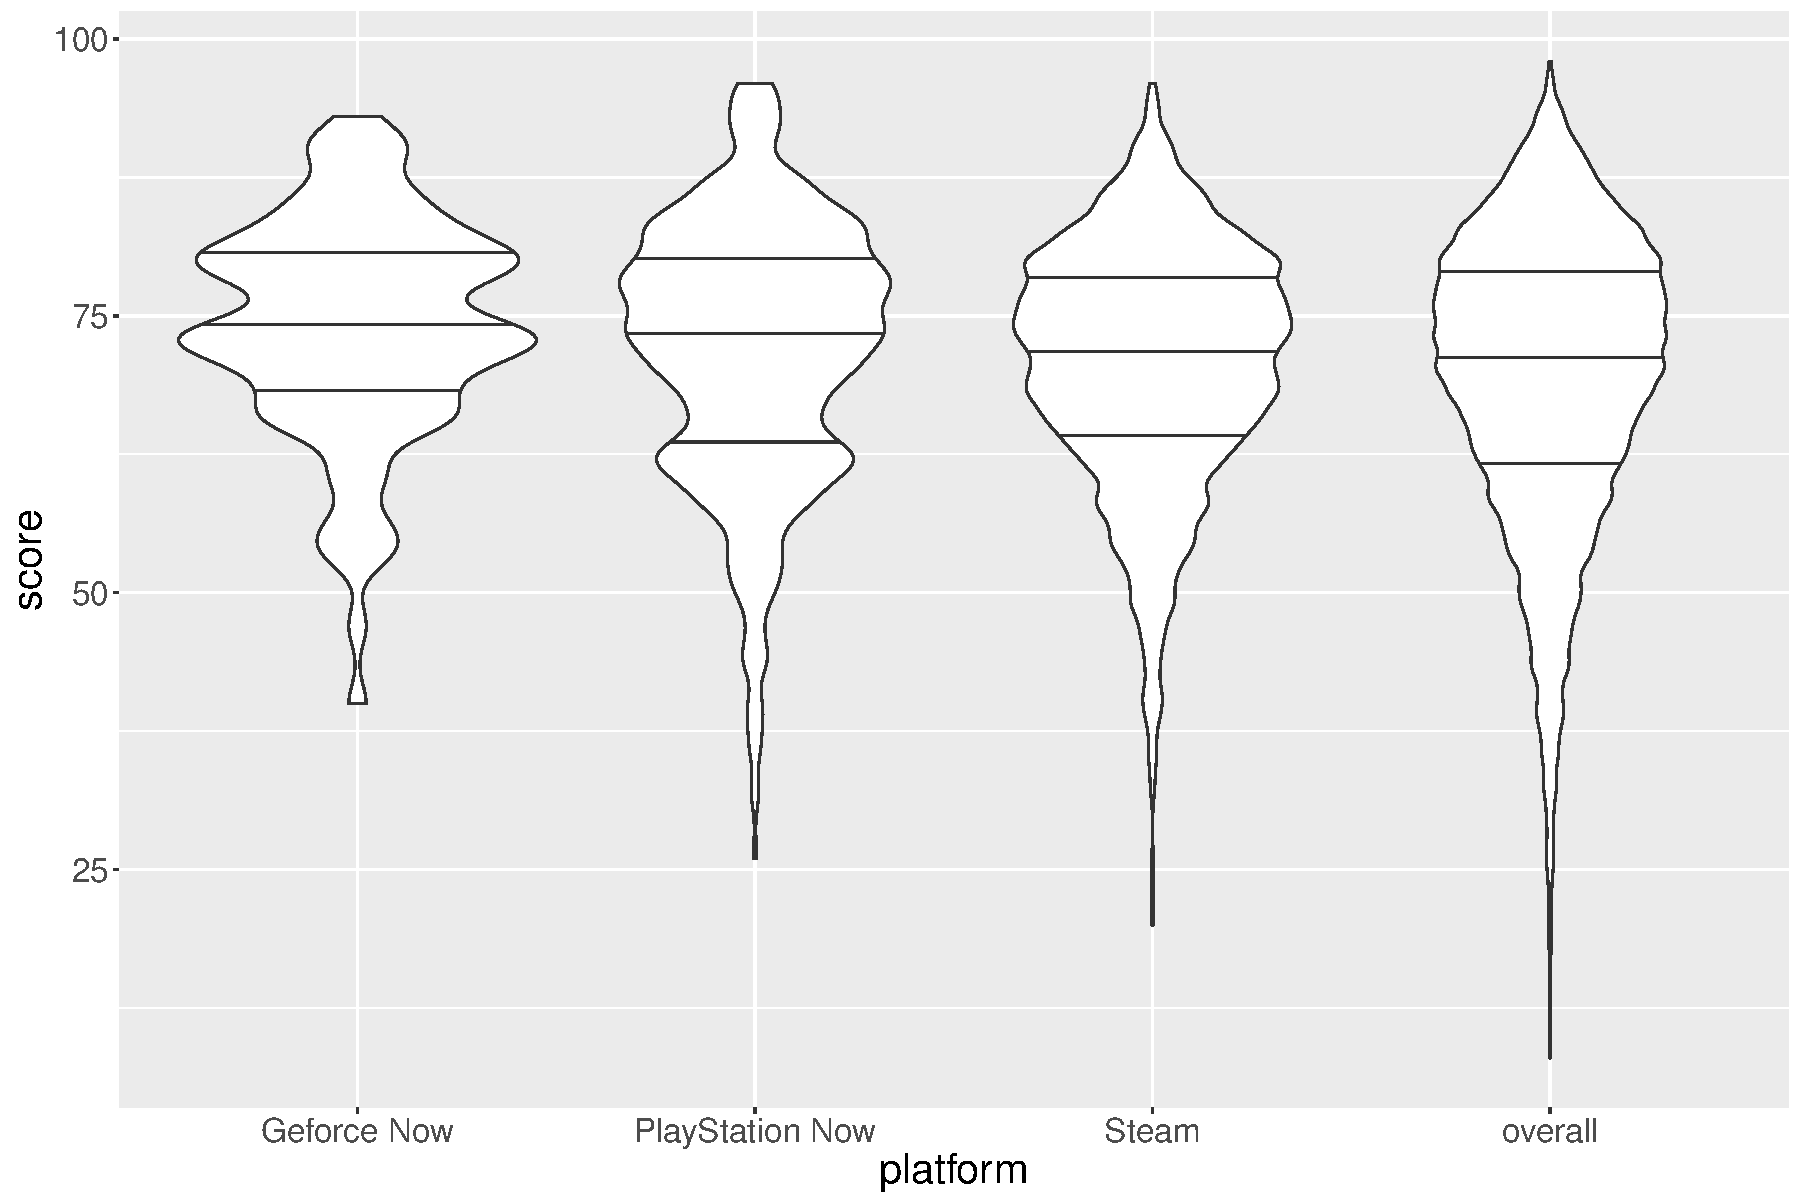
\includegraphics[width=1.0\columnwidth]{images/scores-by-platform-violin.pdf}
	\caption{Distribution of aggregated review scores across the investigated platforms, depicted as violin plot with $25\%$, $50\%$, $75\%$ quantiles drawn.}
\label{fig:scores-by-platform}
\end{figure}

A third examined factor are the review scores as collected in the \metacritic set which seem quite similar across all services, albeit with a slightly lower $\sigma$ for \gfnow. This can probably be attributed to both the small scale and through manual curation. Though, the mean values do not expose the whole picture of review scores, as evident in the violin plots of Fig.~\ref{fig:scores-by-platform}. Both streaming services seem to favor certain score levels. Specifically, they both show a number of highly rated titles, followed by a bulge of average ratings and few but noticeable titles in the low score tail. These could be indications of the different nature of today's cloud gaming ecosystems. \steam on the one side is a more or less open platform, where every game publisher can sell their games at their own volition (platform operator collects a commission fee for sales). Cloud gaming platforms have to acquire licenses from the individual games' publishers and therefore have to be selective and curated by nature. 

A closer look at the \metacritic scores for assessing engagement reveals a small correlation between general score and number of game ownerships on \steam (as an indicator for popularity of a game): Pearson correlation coefficient $= 0.1998204$. Interestingly, for \metacritic user scores the effect turns out to be smaller (Pearson correlation $= 0.1010024$). 
\todo[inline]{PZ: And that tells us what?}

Finally, the length of games is an example of content-based engagement factors. To assume that a longer game might be more engaging to many players might be a viable assessment. But this would need further validation, as it does characterise the quality of the game. As a first indicator the correlation coefficient between number of game ownerships on \steam and combined game length from the \hltb dataset reveal a small effect (Pearson correlation $= 0.175819$, see figure \ref{fig:rel-combinedlength-owners}). Again, all three platforms are rather closely grouped together in this metric, with the one exception being \steam's variance being higher, signifying once again a broader range of available game titles.



\begin{figure}[!t]
	\centering
	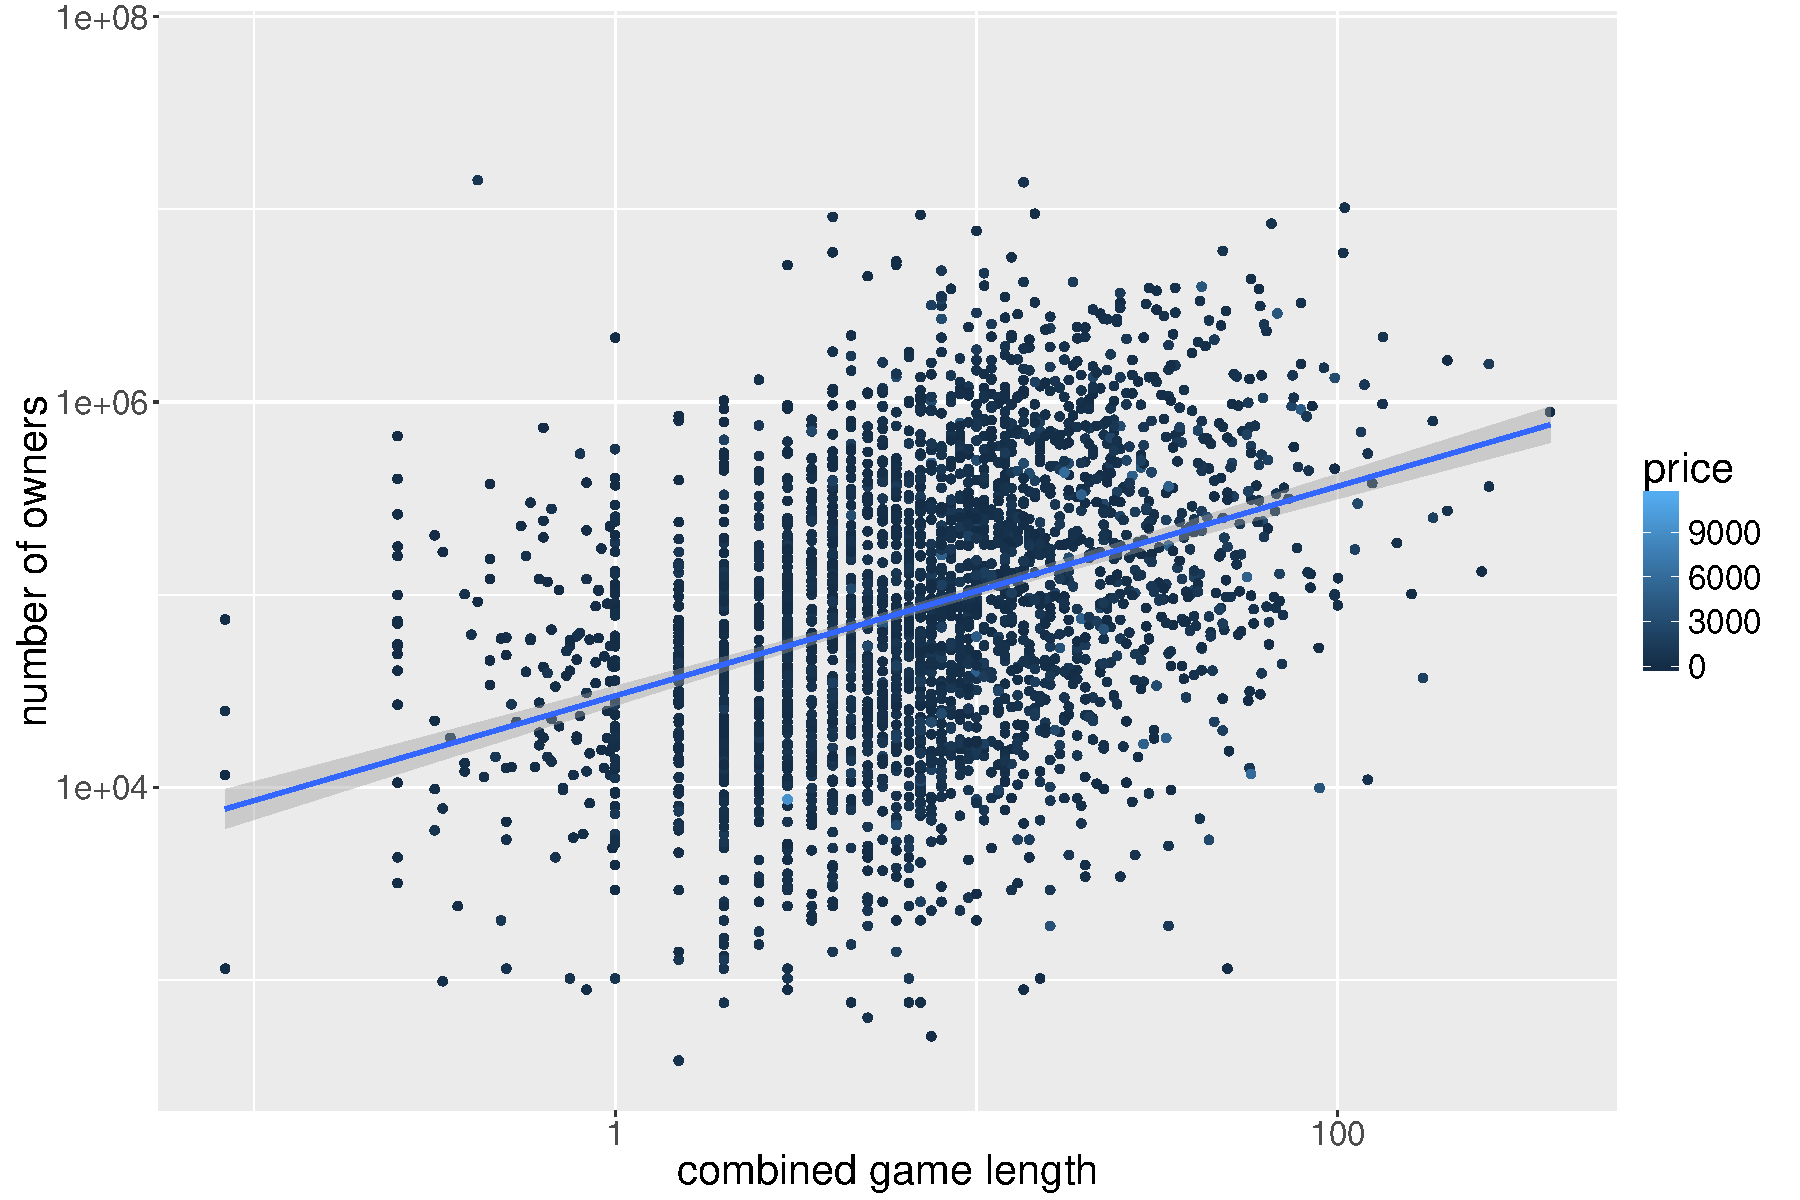
\includegraphics[width=1.0\columnwidth]{images/rel-combinedlength-owners.pdf}
	\caption{Relationship game length to ownership}
\label{fig:rel-combinedlength-owners}
\end{figure}


%%%%%%%%%%%%
\subsubsection{Further Potential Engagement Factors}

Due to the limited amount of available data the number of currently observable potential engagement metrics is restricted. However, many more come to mind and are worth investigating in the future. These could include,

\begin{itemize}
	\item the number of platform ``exclusive'' game titles,
	\item the genre as well as other classifications of games,
	\item the number of game sales and subscriber numbers,
	\item more objective measures of the game's content (e.g. the variety and quality of game mechanics),
	\item technical aspects of games (e.g. the graphical fidelity, the performance, or the precision and responsiveness of controls),
	\item or other content-centric factors based on the games' content.
\end{itemize}




%However, when having a look at figures \ref{fig:rel-price-category-owners} and \ref{fig:rel-score-category-owners}, 
%Some details remain unclear: Despite having a relatively low Metacritic score, especially games within the 11-20 range seem to have quite a number of owners - why? Also, either games for free or expensive games seem to be popular. Maybe this is an indicator for the differentiation between hardcore and casual gamers? (Probably it would be interesting as well to track the price over the years and also weigh the ownership count relatively to a game's age.)

%\begin{figure}[!t]
%	\centering
%	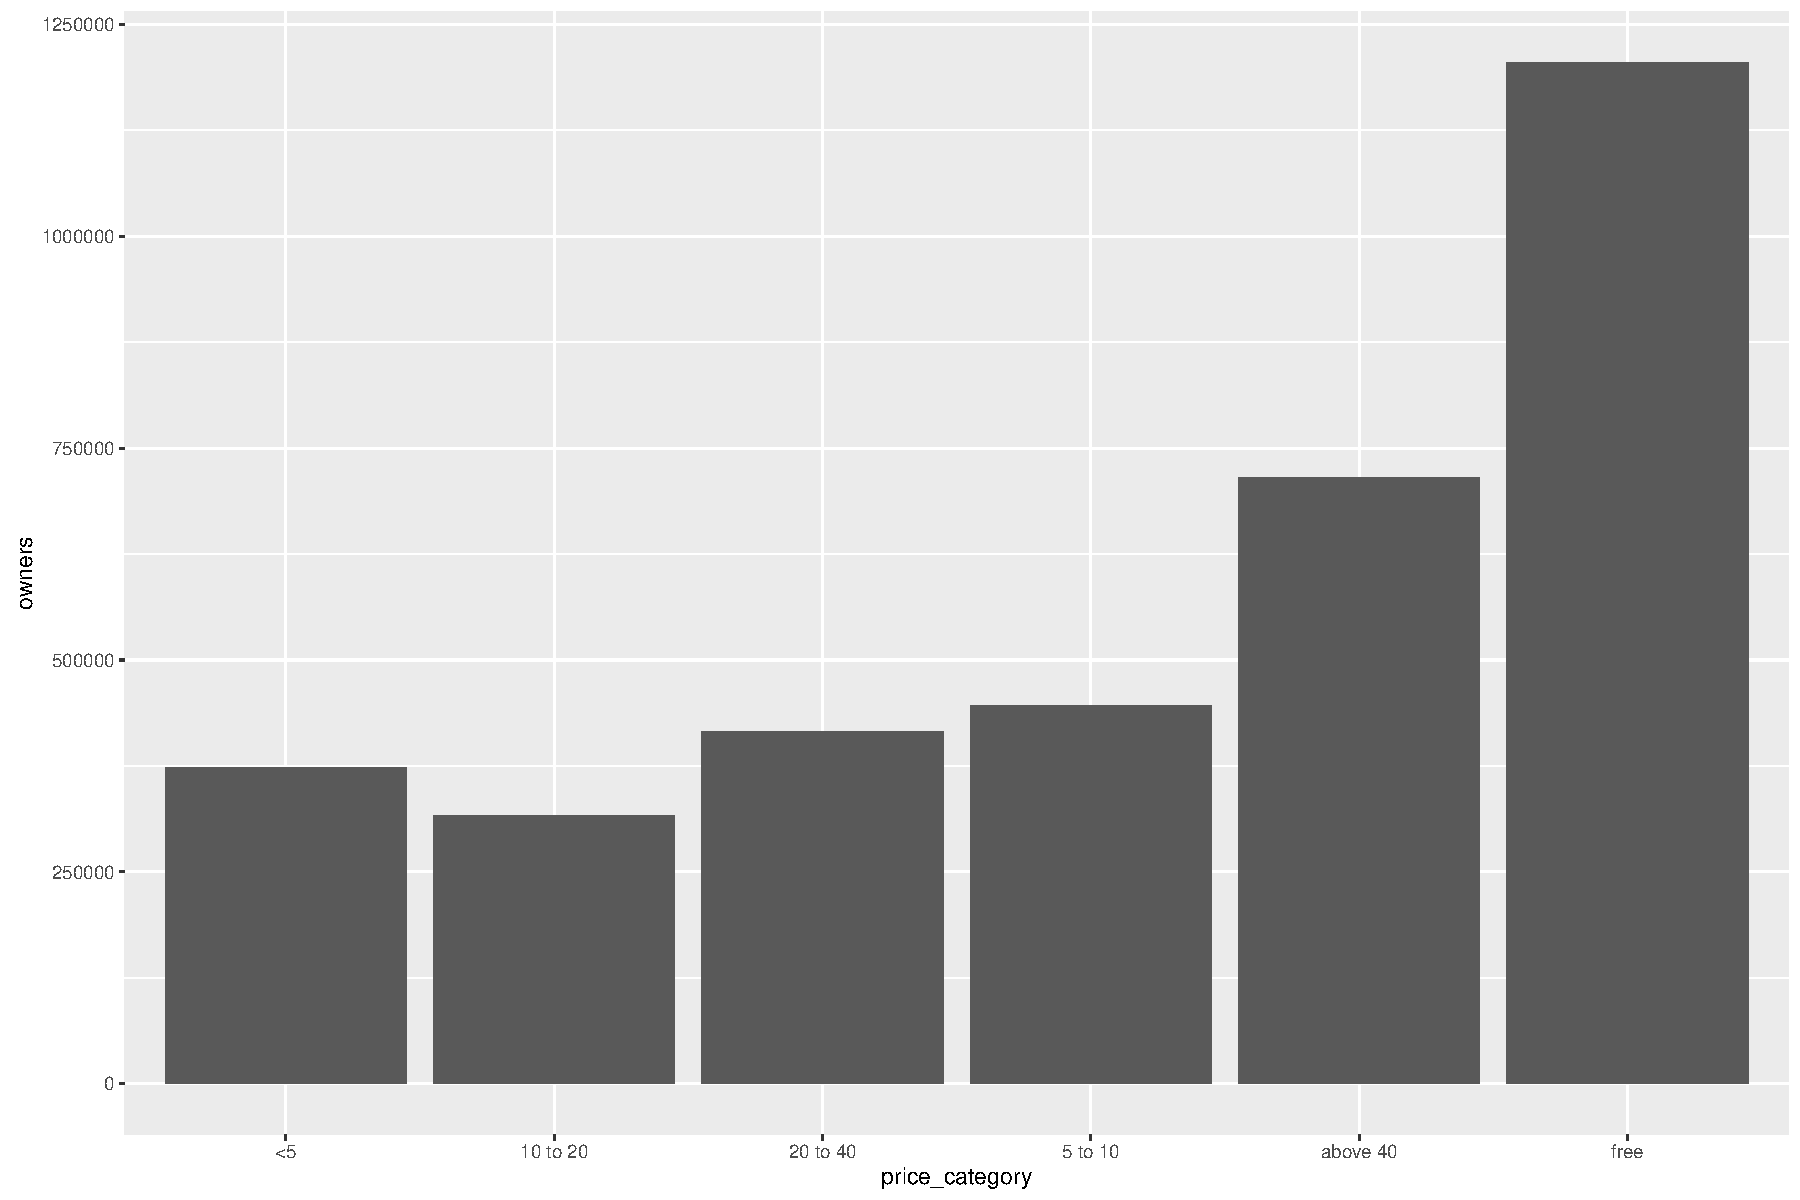
\includegraphics[width=1.0\columnwidth]{images/rel-price-category-owners.pdf}
%	\caption{Relationship price category to ownership (\textbf{TODO: Bars need sorting})}
%\label{fig:rel-price-category-owners}
%\end{figure}
%
%\begin{figure}[!t]
%	\centering
%	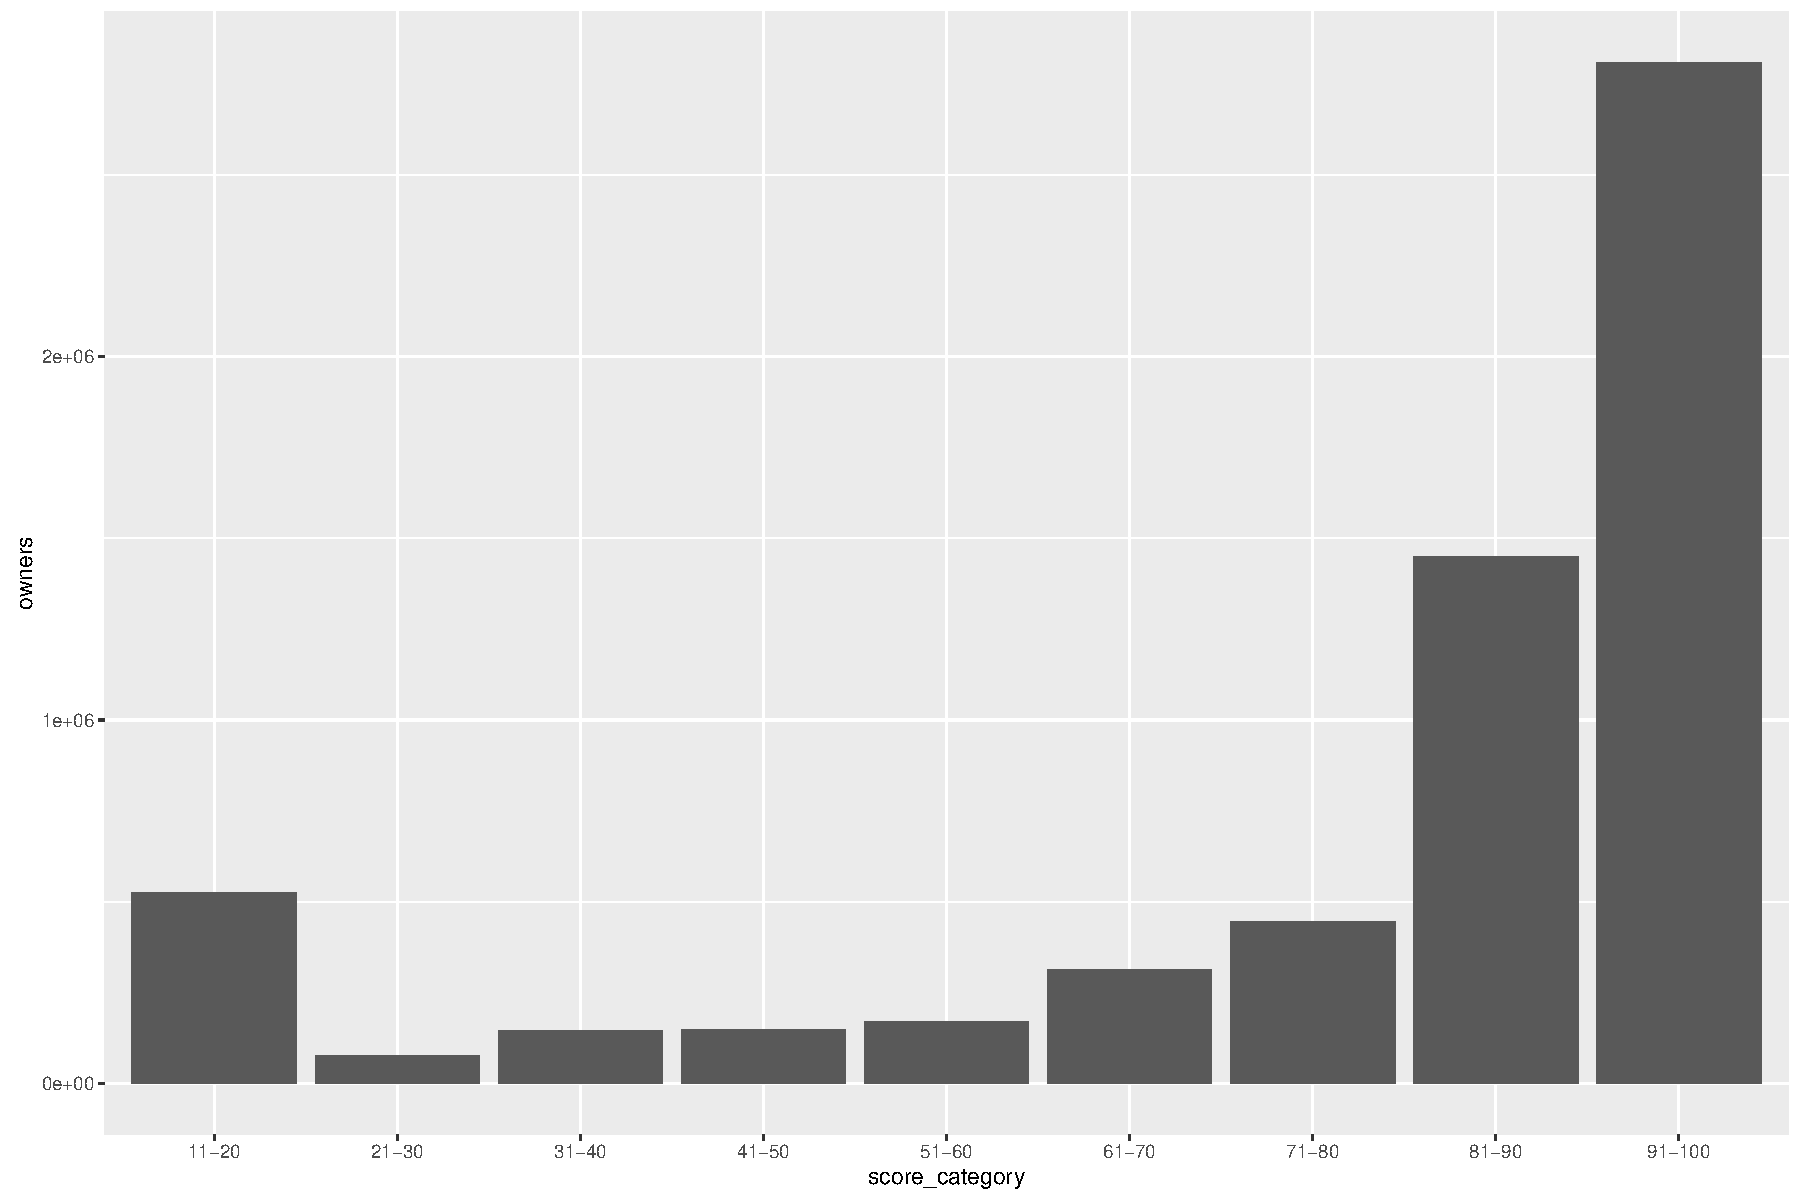
\includegraphics[width=1.0\columnwidth]{images/rel-score-category-owners.pdf}
%	\caption{Relationship score category to ownership (\textbf{TODO: Bars need sorting})}
%\label{fig:rel-score-category-owners}
%\end{figure}


%%%%%%%%%%%%%%%%%%%%%%%%%%%%%%%%%%%%%%%%%%%%%%%%%%%%%%%%%%%%%%%%%%%%%%%%%%%%%%%%
\subsection{Cost-Benefit Models}


The price models for cloud services, as deliberately excluded in the discussion of engagement metrics, largely differ from the approach of \steam. Setting the number of games, as noteworthy value metric, in relationship to the cost or budget (service price), two simple models are created. Naturally, this does not factor in any user preferences to specific games and their availability on just a subset of platforms. But the current curated nature of Cloud Gaming platforms would prevent this endeavour from succeeding regardless.

\todo[inline]{PZ: Which models? Or what are the models?}

%Moreover, the examined engagement metrics do not provide many means for a service distinction bar the number of games available. Therefore, the two simple models provided here use the number of affordable games on a specific budget. 

For both models a few basic assumptions are made. The initial hardware costs are factored in proportionately to the expected life and depreciation time of the devices, which is assumed to be \SI{3}{\year} for PCs and \SI{7}{\year} for the consoles and devices necessary to receive the streaming service (\SI{7}{\year} is about the average life cycle of a video game console generation and should be representative in this case).

What should also be noted is the difference in the service model between the ownership model of \steam, the hybrid subscription plus permanent rental model of \gfnow, as well as the subscription and timed rental model of \psnow. For the latter rentals subscription is also not a prerequisite. As this subtle differences are difficult to express in a simple cost-benefit model, they are all treated the same here. Therefore, they are all treated equally in the models as games, that one has access to and could have been played at one point. Other means of acquiring games cheaper from outside of the respective services, of which there are many for PC gaming as discussed in Sec.~\ref{sec:pcgaming}, are also omitted here.

%%%%%%%%%%%%%%%%%%%%%%%%%%%%%%%%%%%%%%%%%%%%%%
\paragraph{Affordable Games on a Budget Model}

The first model assumes that one has a fixed budget to spend on video games. This model then shows, depending on the size of the budget, how many games one would be able to afford considering all initial and continual costs.

\begin{figure}[!t]
	\centering
	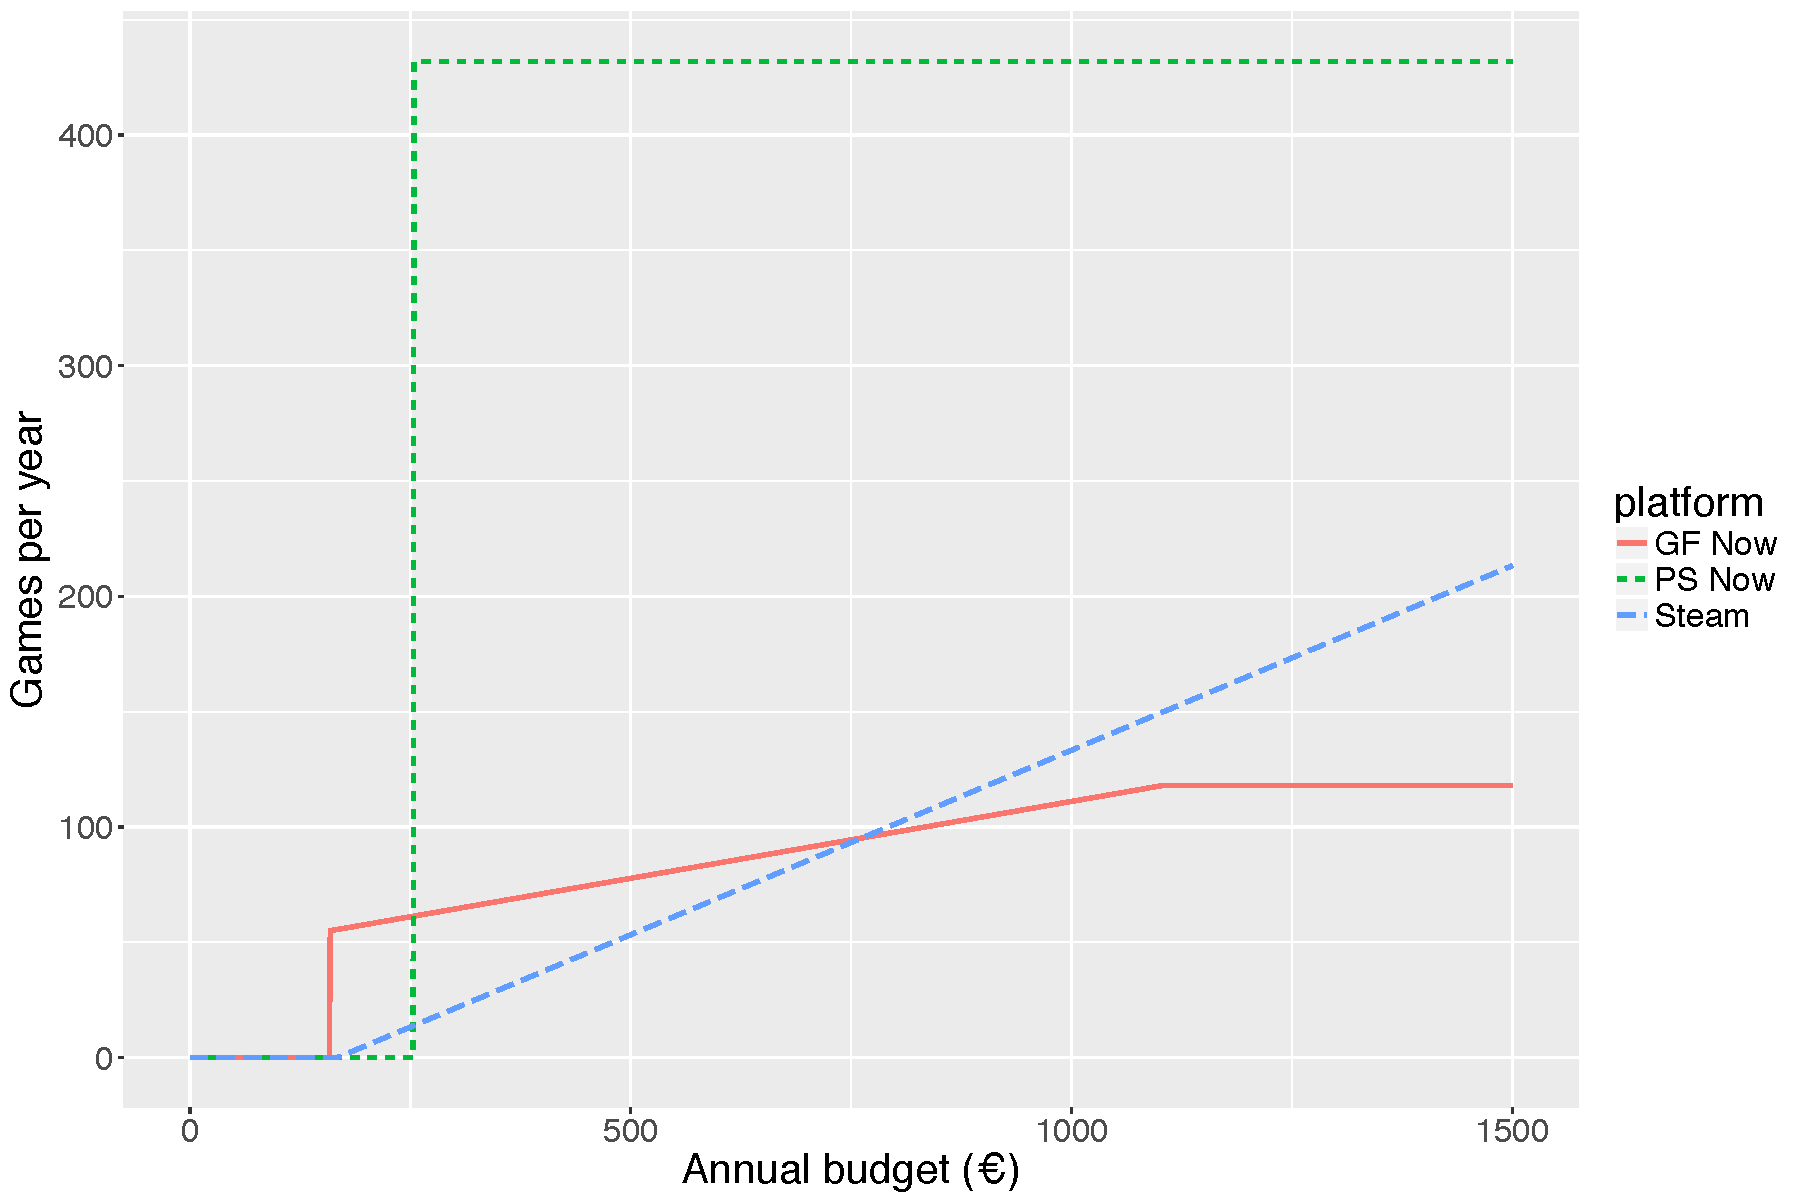
\includegraphics[width=1.0\columnwidth]{images/gamesperyear-over-budget.pdf}
	\caption{Models for several platforms showing the number of games per year that can be bought with a specific budget.}
\label{fig:gamesperyear-over-budget}
\end{figure}

As evident in Fig.~\ref{fig:gamesperyear-over-budget} all platforms start with relatively high fix costs, but only the subscription models provide instant access to a certain amount of titles, which could make them more attractive to newcomers on a low budget. Once one gets more interested in gaming and has access to a somewhat higher budget, the limited nature of both \psnow and \gfnow becomes evident.


%%%%%%%%%%%%%%%%%%%%%%%%%%%%%%%%%%%%%%%%%%%
\paragraph{Affordable Games per Year Model}

The second model extends the previous budget model to a longer time period of several years, investigating the value one gets if only a very low annual budget is spent. For the exemplary model it is assumed to be \SI{500}{\EUR}

\begin{figure}[!t]
	\centering
	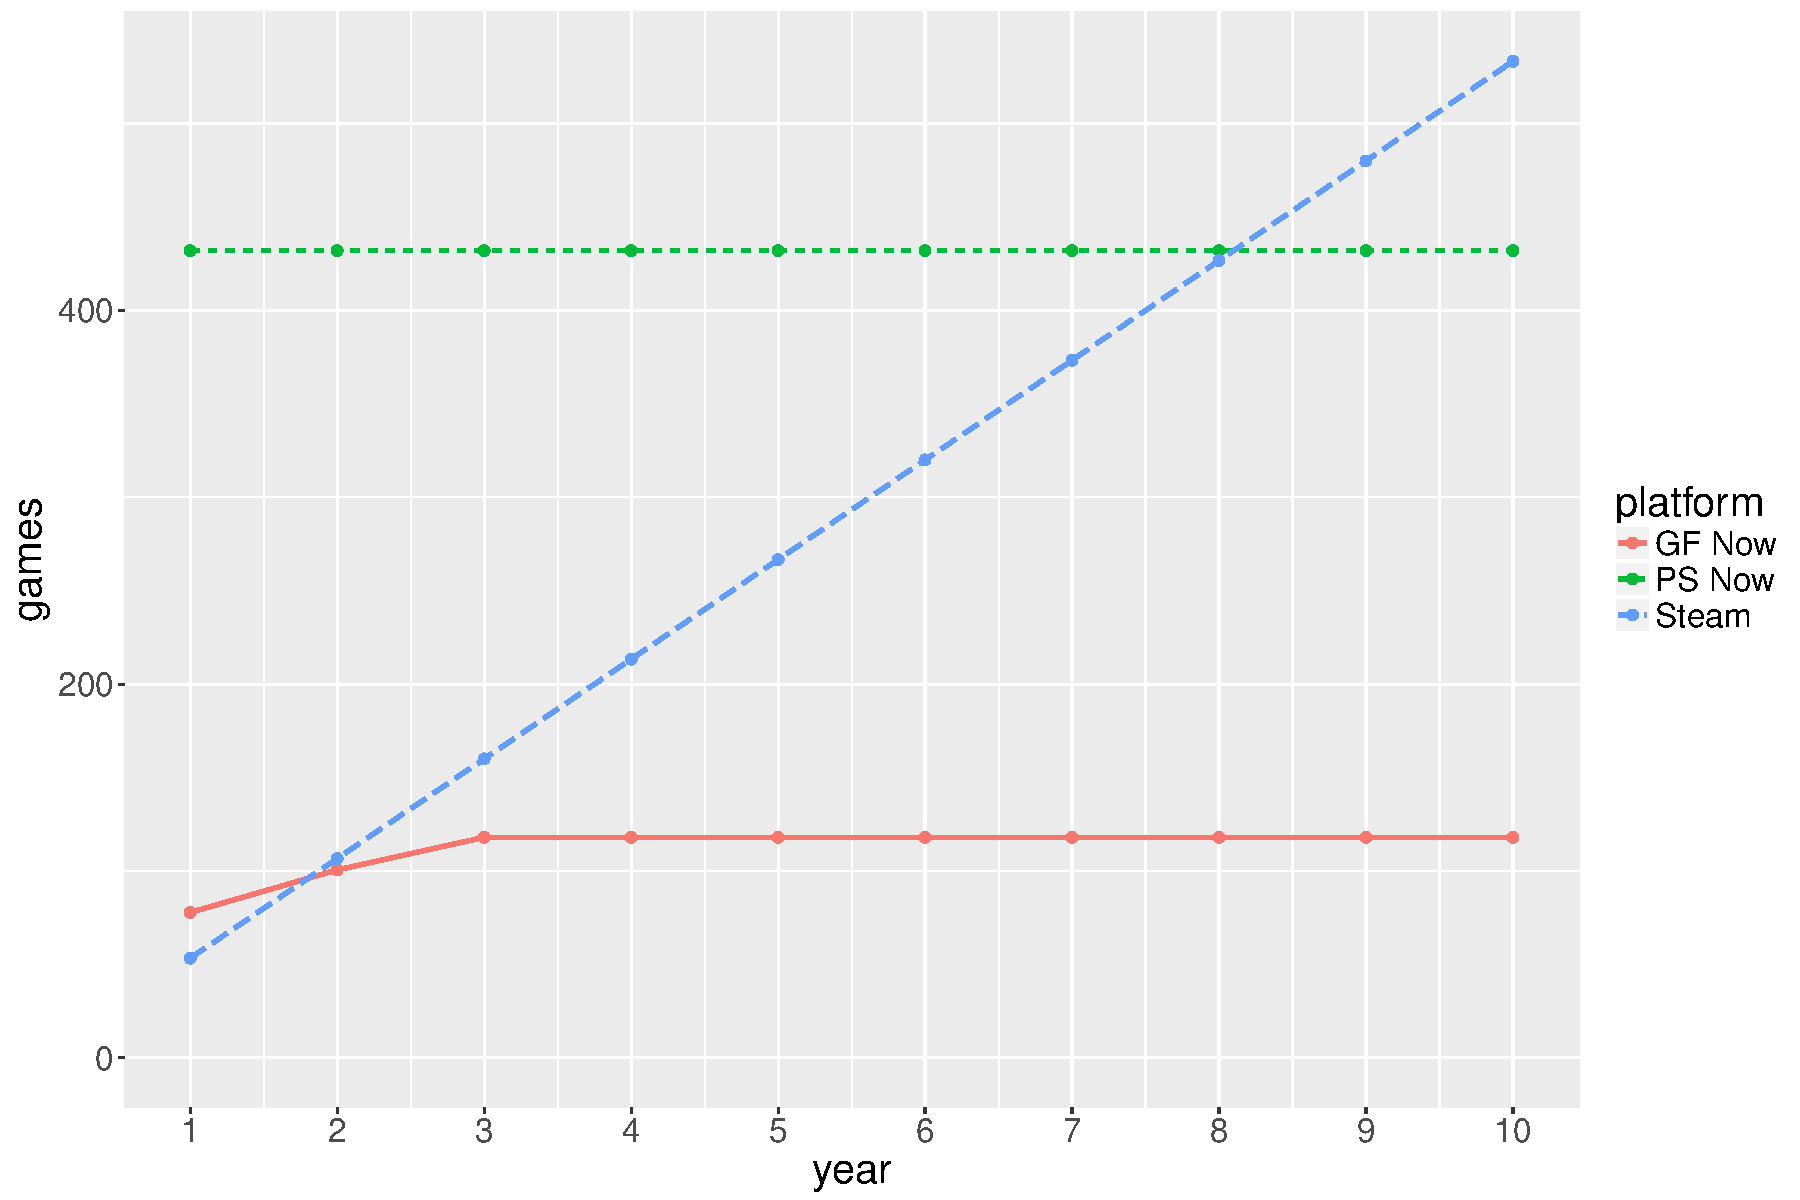
\includegraphics[width=1.0\columnwidth]{images/games-over-year.pdf}
	\caption{Models for several platforms showing the number of games that can be bought over the years subscribed to / using this service.}
\label{fig:games-over-years}
\end{figure}

Fig.~\ref{fig:games-over-years} depicts this example over ten years. The continual subscription costs limit the remaining budget for additional rental titles until the maximum number of titles is reached with that particular service, whereas the number of titles from \steam will just climb steadily. The benefits of a multi-year commitment to these Cloud Gaming services therefore seem to be very limited, especially when considering, that no games are retained after ending the subscription.


%%%%%%%%%%%%%%%%%%%%%%%%%%%%%%%%%%%%%%%%%%%%%%%%%%%%%%%%%%%%%%%%%%%%%%%%%%%%%%%%
\subsection{Discussion}

Summing this section up, the investigated simple engagement metrics somewhat expose the difference between an open market platform and the curated-by-necessity cloud gaming services. The size and sales-based price model of \steam poses challenges for direct competitors such as \gfnow. Services that cater to different audiences, such as \psnow which positions itself as a backwards compatibility service, may have more success in this regard. However, the limited target audience of \psnow becomes even narrower when the high subscription costs are taken into account, diminishing the benefits for many, not even considering the additional quality challenges that streaming video games brings along. All in all this may make curated Cloud Gaming services financially unattractive for the service's operator as is discussed in the following section.

% \todo[inline]{PZ: Ist Grafik \ref{fig:games-over-years} die Basis fuer die Steigung bei ps now usw. ab dem Eintritt in Fig.~\ref{fig:gamesperyear-over-budget}. Ps now wuerde ich als Club Good sehen.}
% \todo[inline]{FM: psnow/clubgood in the sense of a backwards compatibility service for devices that do not have native access to the streamed titles?.}

%PS Now specifically caters towards older titles and backwards compatibility, may find a niche here
% wer ist die zielgruppe?
% was ist die beste platform?
% gibt es eine mainstream platform?
% unterschiedliche ausrichtungen?





% metacritic titles:
% PC 16192
% PS4 817
% XB1 588
% WiiU 474
% 3DS 871
% GFNOW 68
% PSNOW 243
% STEAM 7749



% \begin{figure}[!t]
% 	\centering
% 	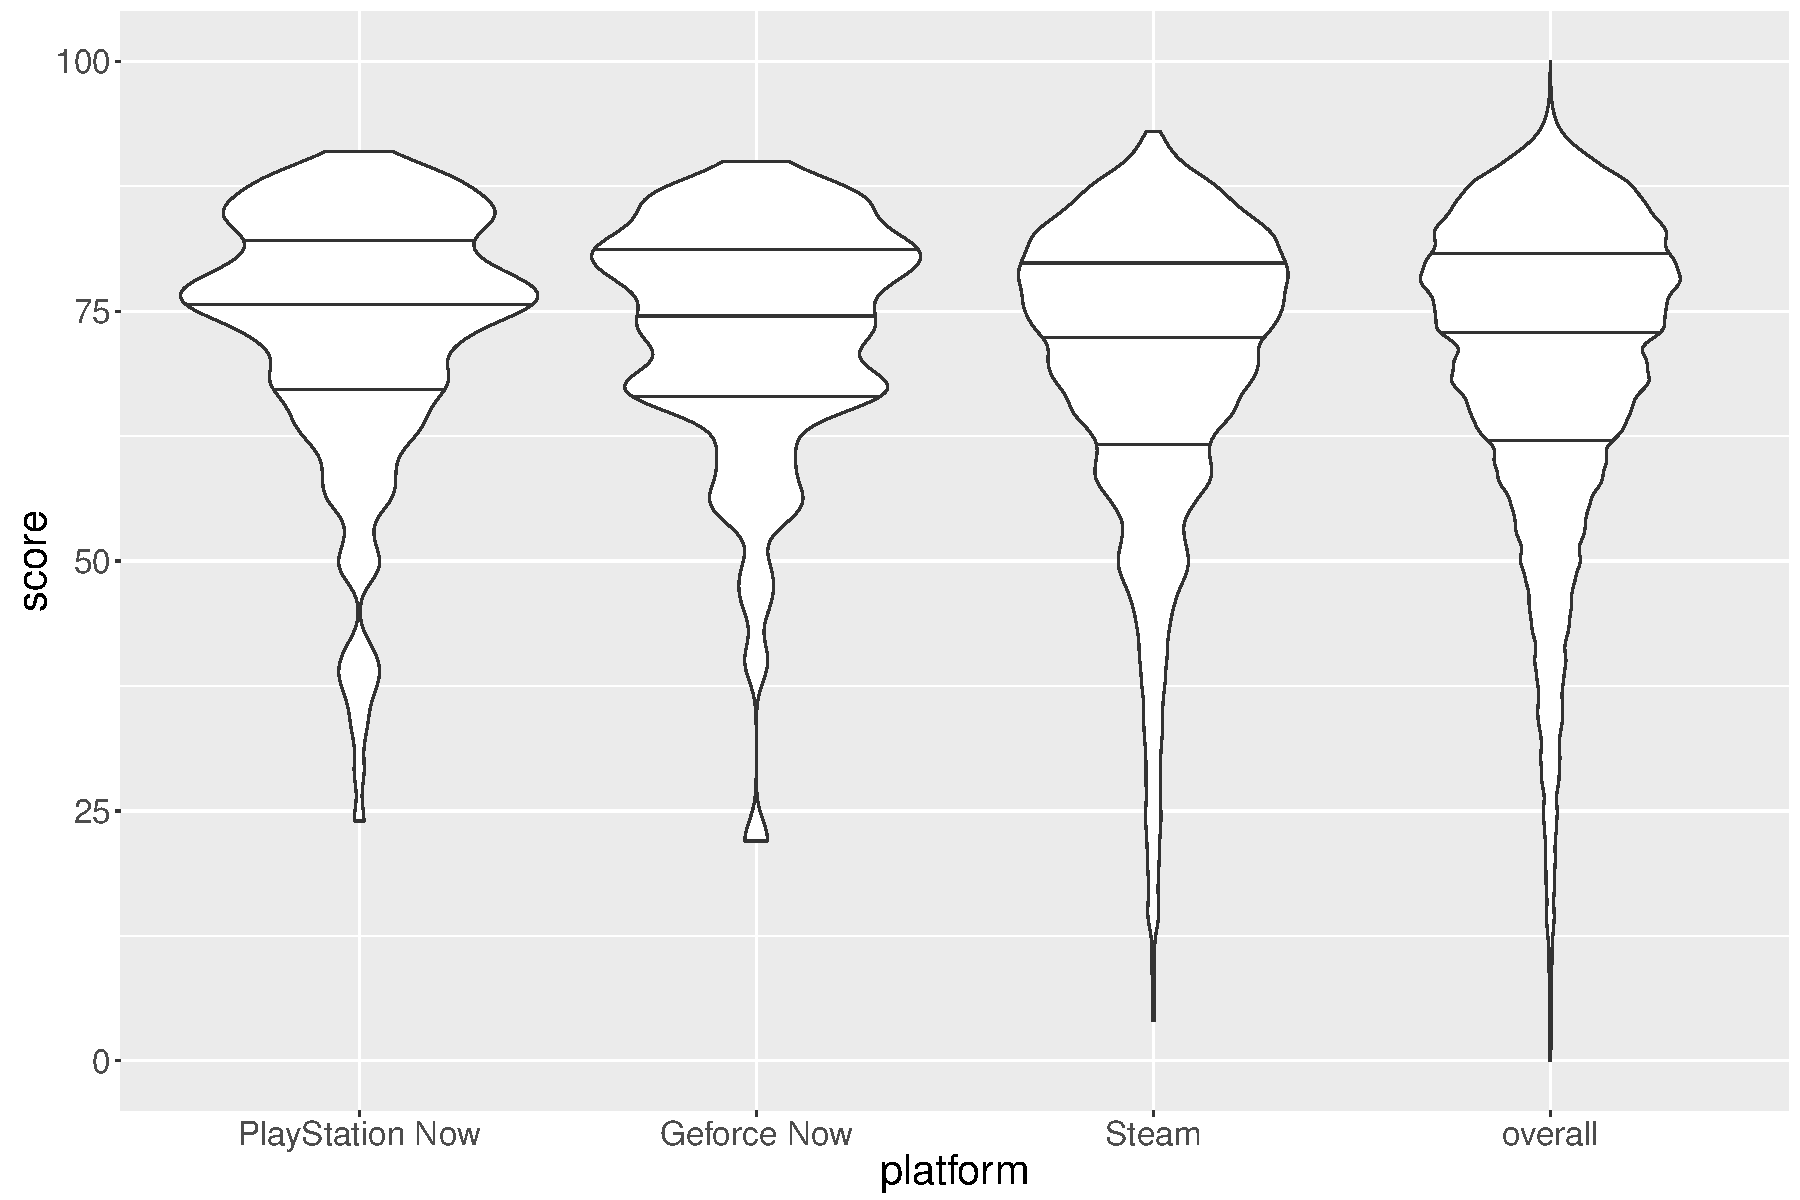
\includegraphics[width=1.0\columnwidth]{images/scores-by-platform-violin-userscore.pdf}
% 	\caption{Distribution of Metacritic user scores across the investigated platforms, depicted as violin plot with $25\%$, $50\%$, $75\%$ quantiles drawn.}
% \label{fig:userscores-by-platform}
% \end{figure}


% \subsection{E2E Lag}
% End-to-End Lag Model and Simulation in R. Now a standalone (submitted) paper at \url{https://github.com/mas-ude/onlinegame-lag-sim}. Can be referenced to argue the need for low E2E lag (meaning low network delay, but also the need for high fps).


%\item Graphical fidelity
%\item , tightness/precision/quality of controls and game mechanics, e2e lag
%\item Story?
%\item Other popularity measures? %(e.g. steamspy owner data?)
%\item Hardware requirements of games?
%\item Game costs and price history



% Caution: 
% Steam means game ownership
% PS/GF Now means only games during subscription plus permanent rental as long the sub is active(?)
% Additionally, PS Now means renting for 30 days